% Provenance (never printed): see sources/outline_sources.md (Year 3: the
% Rayleigh number; thermal boundary layers; slab pull and ridge push; plumes;
% post-glacial rebound and mantle viscosity). Brief: sources/book5/BRIEFS.md,
% ch. 6. Curves from figdata/bachelor-3/convection_scaling.py (PREM read only),
% gia_relaxation.py and ridge_push.py (on plate_cooling.py). Exercise and
% problem values in the Book 5 scratch calculator calc/ch06.py.
\chapter{Mantle Convection and Plate Driving Forces}\label{ch:b3:mantle-convection}

The coast of northern Sweden rises out of the sea by about a centimetre a
year, ten thousand years after the ice sheet that covered it melted away; the
shores of Hudson Bay rise as fast. Nothing pushes them up but the mantle,
slowly flowing back beneath the place the ice had pressed down. The rate at
which the ground springs back weighs the viscosity of the mantle, and the same
viscosity sets how fast the mantle convects and the plates move. This chapter
asks why the solid mantle convects at all, how fast it must flow to carry the
Earth's heat, what forces move the plates, and what the rebound of the ground
says about the mantle's viscosity.
% ledger: vestol19:umea, zhao12:fenno, sella07:gia

\begin{recall}
Viscosity, the creeping flow of a viscous fluid (the Stokes equations
$\nabla p = \eta\nabla^2\mathbf u$, $\nabla\cdot\mathbf u = 0$), Stokes' law
for a sphere, the Reynolds number and buoyancy are in the physics books'
university volumes. Mantle convection and isostatic rebound were met in the
high-school volume (Grade 12), ridge push and slab pull in its Grade 11 part.
The thermal boundary layer, the thermal lithosphere and the mantle adiabat are
in the Year 1 volume, in its chapter on the Earth's heat budget; hotspots,
mantle plumes and large igneous provinces in its chapter on hotspots. The
\omterm{def:b3:lithosphere-thermal-models:half-space}{half-space cooling model} is in \cref{ch:b3:lithosphere-thermal-models},
flexure of the lithosphere in \cref{ch:b3:gravity-geodesy}, \omterm{def:b3:seismology-imaging:tomography}{seismic
tomography} in \cref{ch:b3:seismology-imaging}.
\end{recall}

\section{Why the mantle convects}

The mantle is solid: it carries S waves. Over millions of years, however, it
creeps like a fluid of enormous viscosity, and a layer of fluid heated from
below and cooled from above may stay at rest, the heat crossing it by
conduction, or overturn. A blob of hot fluid of size $d$, lighter than its
surroundings by $\rho\alpha\,\Delta T$, rises at a speed of order
$\rho g\alpha\,\Delta T d^2/\eta$; it loses its heat by diffusion in a time of
order $d^2/\kappa$. If it can rise across the layer before it has cooled, the
layer overturns.

\begin{definition}[Rayleigh number]\label{def:b3:mantle-convection:rayleigh}
For a fluid layer of thickness $d$, density $\rho$, thermal expansion
coefficient $\alpha$, thermal diffusivity $\kappa$ and viscosity $\eta$, under
gravity $g$, with a temperature difference $\Delta T$ between its base and its
top, the \emph{Rayleigh number}\index{Rayleigh number} is
\[
  \mathrm{Ra} = \frac{\rho g\alpha\,\Delta T d^3}{\kappa\eta},
\]
the ratio of the diffusion time $d^2/\kappa$ to the buoyant rise time
$\eta/(\rho g\alpha\,\Delta Td)$.
\end{definition}

\begin{definition}[Critical Rayleigh number]\label{def:b3:mantle-convection:critical}
The \emph{critical Rayleigh number}\index{critical Rayleigh number}
$\mathrm{Ra}_c$ of a layer is the value of the \omterm{def:b3:mantle-convection:rayleigh}{Rayleigh number} above which a
small disturbance of the state of rest grows into convection, and below which
it dies away.
\end{definition}

\begin{proposition}[Onset of convection]\label{prop:b3:mantle-convection:onset}
For a layer whose top and bottom are free of shear stress and held at fixed
temperatures, a disturbance of horizontal wavenumber $k$ (in units of $1/d$)
grows when $\mathrm{Ra} > (\pi^2 + k^2)^3/k^2$. The minimum of the right-hand
side, at $k = \pi/\sqrt2$, gives
\[
  \mathrm{Ra}_c = \frac{27\pi^4}{4} \approx 657.5,
\]
and the first cells to appear are $2\sqrt2\,d$ wide. Between rigid boundaries,
$\mathrm{Ra}_c \approx 1708$.
\end{proposition}

\admitted
The linear stability analysis behind it, a perturbation of the heat and Stokes
equations about the conductive state, is in the physics books' treatment of
convection; exercise 11 checks the minimum.

The figure below shows the convecting layer. The mantle's values, with the
depth of the core--mantle boundary, $d = \qty{2891}{km}$, the mean density of
the mantle, \qty{4476}{kg.m^{-3}}, and $g$ between 9.8 and
\qty{10.7}{m.s^{-2}}, all from the seismic Earth model PREM; $\alpha =
\qty{3.1e-5}{K^{-1}}$ and $\Delta T = \qty{1450}{K}$ from the plate model of
\cref{ch:b3:lithosphere-thermal-models}; $\kappa = \qty{e-6}{m^2.s^{-1}}$;
and $\eta$ between \num{e21} and \qty{e22}{Pa.s} (\cref{sec:b3:mantle-convection:gia}),
give $\mathrm{Ra}$ between \num{4.9e6} and \num{4.9e7}, some seven thousand to
seventy thousand times critical. The mantle cannot help convecting.
% ledger: data:prem, honda04:gdh1, delaney86:properties, mitrovica96:haskell, milne04:bifrost

\begin{omfigure}
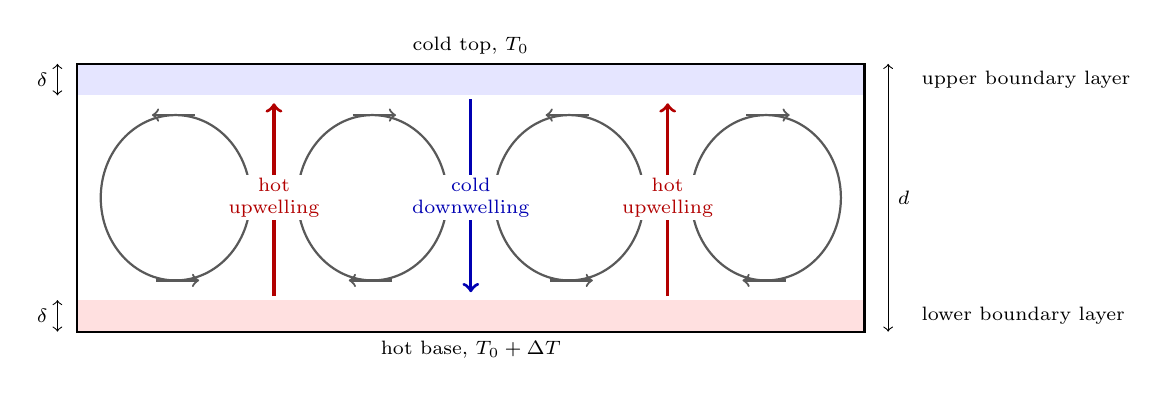
\begin{tikzpicture}[font=\scriptsize, x=1cm, y=1cm]
\fill[blue!10] (0,3.4) rectangle (10,3.0);
\fill[red!12] (0,0) rectangle (10,0.4);
\draw[thick] (0,0) rectangle (10,3.4);
\node[above] at (5,3.4) {cold top, $T_0$};
\node[below] at (5,0) {hot base, $T_0 + \Delta T$};
\foreach \c/\s in {1.25/1, 3.75/-1, 6.25/1, 8.75/-1} {
  \draw[gray!70!black, thick] (\c,1.7) ellipse[x radius=0.95, y radius=1.05];
  \draw[->, gray!70!black, thick] ({\c+0.25*\s},2.75) -- ({\c-0.3*\s},2.75);
  \draw[->, gray!70!black, thick] ({\c-0.25*\s},0.65) -- ({\c+0.3*\s},0.65);
}
\draw[->, red!70!black, very thick] (2.5,0.45) -- (2.5,2.9);
\draw[->, red!70!black, very thick] (7.5,0.45) -- (7.5,2.9);
\draw[->, blue!70!black, very thick] (5,2.95) -- (5,0.5);
\node[red!70!black, fill=white, inner sep=1pt, align=center] at (2.5,1.7) {hot\\upwelling};
\node[red!70!black, fill=white, inner sep=1pt, align=center] at (7.5,1.7) {hot\\upwelling};
\node[blue!70!black, fill=white, inner sep=1pt, align=center] at (5,1.7) {cold\\downwelling};
\draw[<->] (10.3,0) -- (10.3,3.4) node[midway, right] {$d$};
\draw[<->] (-0.25,3.0) -- (-0.25,3.4) node[midway, left] {$\delta$};
\draw[<->] (-0.25,0) -- (-0.25,0.4) node[midway, left] {$\delta$};
\node[anchor=west] at (10.6,3.2) {upper boundary layer};
\node[anchor=west] at (10.6,0.2) {lower boundary layer};
\end{tikzpicture}

\par\smallskip{\small Convection in a layer heated from below and cooled from
above. Heat crosses the thin boundary layers, of thickness $\delta$, by
conduction; in between, the well-mixed interior carries it by flow. Cold sheets
detach from the upper layer and sink; hot ones rise from the
lower.}\label{fig:b3:mantle-convection:cell}
\end{omfigure}

The mantle is also heated from within, by the decay of radioactive elements,
and from below, by the core. A layer heated only from within has no hot
boundary layer at its base: its flow is driven by cold sheets sinking from the
top, the rising flow being a broad, passive return. Slabs are such sheets, and
plumes need the heat from the core.

\section{Boundary layers and the strength of convection}

\begin{definition}[Nusselt number]\label{def:b3:mantle-convection:nusselt}
The \emph{Nusselt number}\index{Nusselt number} of a convecting layer is the
heat flow through it divided by the heat flow that conduction alone would carry
across the same layer, $\mathrm{Nu} = q\,d/(k\,\Delta T)$.
\end{definition}

\begin{theorem}[Boundary-layer scaling of convection]\label{thm:b3:mantle-convection:scaling}
In a layer convecting at $\mathrm{Ra} \gg \mathrm{Ra}_c$, if each thermal
boundary layer grows until its own \omterm{def:b3:mantle-convection:rayleigh}{Rayleigh number}, built on its thickness
$\delta$ and the temperature drop $\Delta T/2$ across it, reaches
$\mathrm{Ra}_c$, then
\[
  \delta = d\Bigl(\frac{2\mathrm{Ra}_c}{\mathrm{Ra}}\Bigr)^{1/3},\qquad
  \mathrm{Nu} = \frac12\Bigl(\frac{\mathrm{Ra}}{2\mathrm{Ra}_c}\Bigr)^{1/3},
  \qquad
  u = \frac\kappa d\Bigl(\frac{\mathrm{Ra}}{2\mathrm{Ra}_c}\Bigr)^{2/3},
\]
where $u$ is the velocity scale of the flow, defined by requiring that the
layer grows to $\delta$ while the fluid crosses the cell. This is the
\emph{boundary-layer scaling of convection}\index{boundary-layer scaling of convection}.
\end{theorem}

\begin{proof}
The interior is well mixed, at the mean temperature, so each boundary layer
carries half of $\Delta T$. Its \omterm{def:b3:mantle-convection:rayleigh}{Rayleigh number} is $\rho g\alpha(\Delta T/2)
\delta^3/(\kappa\eta) = \mathrm{Ra}\,(\delta/d)^3/2$; setting it equal to
$\mathrm{Ra}_c$ gives $\delta$. The heat flow is conducted across the layer,
$q = k(\Delta T/2)/\delta$, so $\mathrm{Nu} = qd/(k\Delta T) = d/(2\delta)$.
A boundary layer grows by diffusion to the thickness $\delta$ in a time
$\delta^2/\kappa$; the fluid at the top crosses the cell, of width of order
$d$, in a time $d/u$. Equating the two times, $u = \kappa d/\delta^2 =
(\kappa/d)(d/\delta)^2$.
\end{proof}

The heat flow grows only as the cube root of $\mathrm{Ra}$: a hundred times
lower viscosity, less than five times more heat. With the mantle's
$\mathrm{Ra} = \num{4.9e7}$, the scaling gives $\delta \approx \qty{87}{km}$,
$\mathrm{Nu} \approx 17$, a heat flow of $\mathrm{Nu}\,k\Delta T/d \approx
\qty{26}{mW.m^{-2}}$ with $k = \qty{3.1}{W.m^{-1}.K^{-1}}$, and $u \approx
\qty{1.2}{cm/yr}$ (figure below). The boundary layer is as thick as the
oceanic plate of \cref{ch:b3:lithosphere-thermal-models}, \qty{95}{km}; the
root-mean-square speeds of today's plates range from \qty{1.1}{cm/yr} (South
America) to \qty{7.5}{cm/yr} (Cocos), \qty{4.4}{cm/yr} for the whole
lithosphere. The Earth's mean heat flow, \qty{92}{mW.m^{-2}}, is three to four
times the scaling's: the heat produced within the mantle, which a layer
heated from below leaves out, and the constants of order one that the scaling
ignores both weigh in. For a law with a single input, the orders of magnitude
are right: plates are the upper boundary layer of a mantle with $\mathrm{Ra}
\sim 10^7$.
% ledger: nnr56:rms, b2dd10:continents, honda04:gdh1

\begin{omfigure}
\begin{tikzpicture}
\begin{groupplot}[group style={group size=1 by 2, vertical sep=2.5cm},
  omrecord, width=0.86\linewidth, height=0.40\linewidth, xmode=log, ymode=log,
  xmin=100, xmax=1e10, xlabel={Rayleigh number $\mathrm{Ra}$}]
\nextgroupplot[ylabel={Nusselt number}, ymin=0.3, ymax=300,
  title={(a) heat flow, in units of the conductive flow}, title style={font=\small}]
% computed in figdata/bachelor-3/convection_scaling.py; ledger: data:prem, honda04:gdh1
\addplot[omDef, thick] table[x=ra, y=nu] {figdata/out/bachelor-3-convection_scaling-conduction.dat};
\addplot[red!70!black, thick] table[x=ra, y=nu] {figdata/out/bachelor-3-convection_scaling-scaling.dat};
\addplot[gray, densely dashed, unbounded coords=jump] table[x=ra, y=y] {figdata/out/bachelor-3-convection_scaling-band.dat};
\draw[gray, densely dotted] (axis cs:657.5,0.3) -- (axis cs:657.5,1);
\node[font=\scriptsize, anchor=west] at (axis cs:700,0.45) {$\mathrm{Ra}_c$};
\node[font=\scriptsize, anchor=south west, omDef] at (axis cs:115,1.08) {conduction};
\node[font=\scriptsize, anchor=north west, red!70!black] at (axis cs:3e4,0.95) {$\tfrac12(\mathrm{Ra}/2\mathrm{Ra}_c)^{1/3}$};
\node[font=\scriptsize, fill=white, inner sep=1pt] at (axis cs:1.55e7,120) {mantle};
\nextgroupplot[ylabel={velocity (\unit{cm/yr})}, ymin=1e-3, ymax=100,
  title={(b) velocity scale for $d = \qty{2891}{km}$}, title style={font=\small}]
\addplot[red!70!black, thick] table[x=ra, y=u] {figdata/out/bachelor-3-convection_scaling-scaling.dat};
\addplot[gray, densely dashed, unbounded coords=jump] table[x=ra, y=y] {figdata/out/bachelor-3-convection_scaling-band.dat};
\addplot[blue!70, thick, dash dot, unbounded coords=jump] table[x=ra, y=u] {figdata/out/bachelor-3-convection_scaling-plates.dat};
\node[font=\scriptsize, anchor=south west, blue!60!black] at (axis cs:150,7.6) {fastest plate};
\node[font=\scriptsize, anchor=north west, blue!60!black] at (axis cs:150,1.0) {slowest plate};
\node[font=\scriptsize, fill=white, inner sep=1pt] at (axis cs:1.55e7,0.004) {mantle};
\end{groupplot}
\end{tikzpicture}

\par\smallskip{\small Convection scaling. (a) Below $\mathrm{Ra}_c$ the layer
conducts ($\mathrm{Nu} = 1$); far above it, the boundary-layer law, drawn
from $\mathrm{Ra} = 16\,\mathrm{Ra}_c \approx \num{1.1e4}$, where it gives $\mathrm{Nu} = 1$ (in between,
convection sets in gradually). (b) The velocity
scale for the depth of the mantle and $\kappa = \qty{e-6}{m^2.s^{-1}}$, with the
range of today's plate speeds (dash-dotted). The dashed lines bound the mantle's
\omterm{def:b3:mantle-convection:rayleigh}{Rayleigh number} for viscosities of \num{e22} and \qty{e21}{Pa.s}.}\label{fig:b3:mantle-convection:scaling}
\end{omfigure}

\section{The forces on a plate}

A plate moves at a steady speed: the forces on it balance. Three drive it or
resist it from its edges and its base (figure below). The force that the
sinking slab exerts on its plate, slab pull, comes from the excess density of
a cold slab in the warmer mantle. Ridge push, the push of the high, hot ridge
on the cooler plate beside it, follows from the half-space model of
\cref{ch:b3:lithosphere-thermal-models}.

\begin{omfigure}
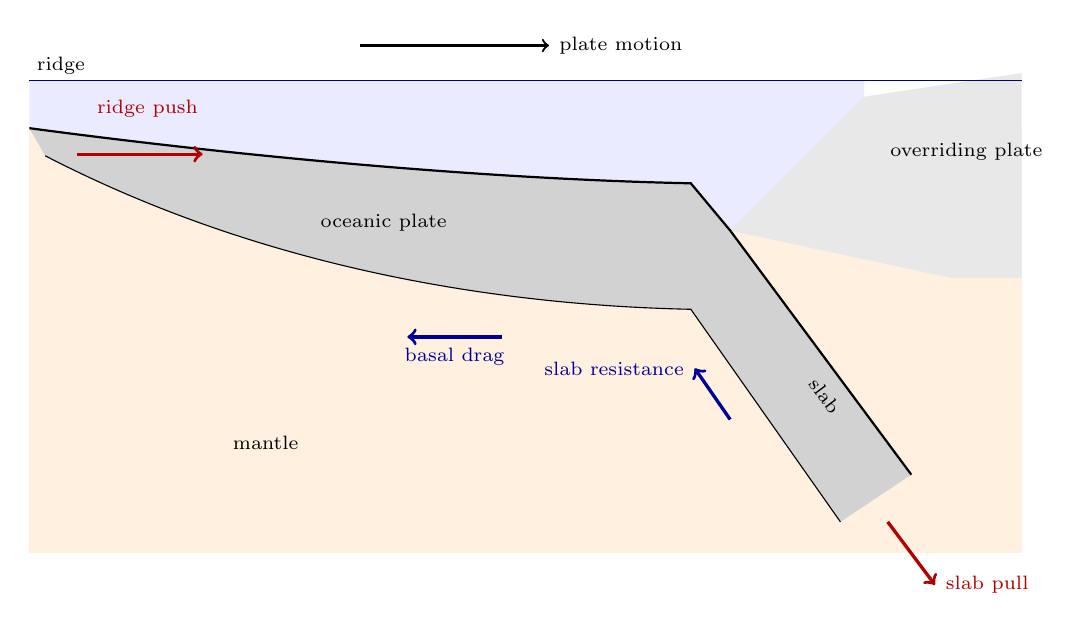
\begin{tikzpicture}[font=\scriptsize, x=1cm, y=1cm]
\fill[orange!12] (0,-0.6) rectangle (12.6,-6.0);
\fill[blue!8] (0,0) -- (0,-0.6) .. controls (3,-1.0) and (6,-1.25) .. (8.4,-1.3) -- (8.9,-1.9) -- (10.6,-0.2) -- (10.6,0) -- cycle;
\fill[gray!35] (0,-0.6) .. controls (3,-1.0) and (6,-1.25) .. (8.4,-1.3) -- (8.9,-1.9) -- (11.2,-5.0) -- (10.3,-5.6) -- (8.4,-2.9) .. controls (6,-2.85) and (3,-2.4) .. (0.2,-0.95) -- cycle;
\fill[gray!18] (10.6,-0.2) -- (12.6,0.1) -- (12.6,-2.5) -- (11.7,-2.5) -- (8.9,-1.9) -- cycle;
\draw[thick] (0,-0.6) .. controls (3,-1.0) and (6,-1.25) .. (8.4,-1.3) -- (8.9,-1.9) -- (11.2,-5.0);
\draw (0.2,-0.95) .. controls (3,-2.4) and (6,-2.85) .. (8.4,-2.9) -- (10.3,-5.6);
\draw[blue!50!black] (0,0) -- (12.6,0);
\node at (0.4,0.2) {ridge};
\node at (4.5,-1.8) {oceanic plate};
\node at (11.9,-0.9) {overriding plate};
\node[rotate=-53] at (10.1,-4.0) {slab};
\node at (3,-4.6) {mantle};
\draw[->, very thick, red!70!black] (0.6,-0.93) -- (2.2,-0.93);
\node[red!70!black] at (1.5,-0.35) {ridge push};
\draw[->, very thick, red!70!black] (10.9,-5.6) -- (11.5,-6.4) node[right] {slab pull};
\draw[->, very thick, blue!60!black] (6.0,-3.25) -- (4.8,-3.25) node[below, pos=0.5] {basal drag};
\draw[->, very thick, blue!60!black] (8.9,-4.3) -- (8.45,-3.65) node[left] {slab resistance};
\draw[->, thick] (4.2,0.45) -- (6.6,0.45) node[right] {plate motion};
\end{tikzpicture}

\par\smallskip{\small The forces on an oceanic plate: ridge push and slab pull
drive it (red); drag at its base, where the plate moves faster than the mantle
beneath, and the viscous resistance of the mantle to the sinking slab resist
it (blue).}\label{fig:b3:mantle-convection:forces}
\end{omfigure}

\begin{proposition}[Ridge-push force]\label{prop:b3:mantle-convection:ridge-push}
In the \omterm{def:b3:lithosphere-thermal-models:half-space}{half-space cooling model}, with mantle temperature $T_m$, surface
temperature $T_0$ and isostatic compensation, the horizontal force per unit
length of ridge that the column at the ridge exerts on the plate of age $t$,
the \emph{ridge-push force}\index{ridge-push force}, is
\[
  F_{rp} = g\rho_m\alpha(T_m - T_0)\kappa t\Bigl[1 + \frac{2\rho_m\alpha(T_m
  - T_0)}{\pi(\rho_m - \rho_w)}\Bigr].
\]
\end{proposition}

\begin{proof}
Let $y$ be the depth below the sea floor at the ridge, $w$ the subsidence of
the floor of age $t$, $\theta(z) = T_m - T(z)$ the temperature deficit at the
depth $z = y - w$ in its plate, and $\Theta(z) = \int_0^z\theta$. The ridge
column holds mantle of density $\rho_m$ from $y = 0$; the old column holds
water down to $w$, then plate of density $\rho_m(1 + \alpha\theta)$. The
lithostatic pressures differ by $P_r - P_t = (\rho_m - \rho_w)gy$ for $y < w$,
and below,
\[
  P_r - P_t = (\rho_m - \rho_w)gw - \rho_mg\alpha\,\Theta(z)
  = \rho_mg\alpha\bigl(\Theta(\infty) - \Theta(z)\bigr),
\]
by isostasy, $(\rho_m - \rho_w)w = \rho_m\alpha\Theta(\infty)$. The force is the
integral of the pressure difference over depth; integrating the second part by
parts,
\[
  F_{rp} = \tfrac12(\rho_m - \rho_w)gw^2 + \rho_mg\alpha\int_0^\infty
  z\,\theta(z)\,\mathrm dz .
\]
For the half-space, $\theta = (T_m - T_0)\operatorname{erfc}(z/2\sqrt{\kappa
t})$ and $\int_0^\infty x\operatorname{erfc}x\,\mathrm dx = 1/4$, so the
integral is $(T_m - T_0)\kappa t$; and $w = 2\rho_m\alpha(T_m -
T_0)\sqrt{\kappa t/\pi}/(\rho_m - \rho_w)$. Adding the two terms gives the
formula.
\end{proof}

Ridge push grows linearly with age: it is not a push at the axis but a
pressure gradient spread over the whole cooling plate. With the values of
\cref{ch:b3:lithosphere-thermal-models}, the bracket is 1.04 and $F_{rp} =
\qty{3.8e12}{N.m^{-1}}$ at \qty{100}{Myr}. In the plate model it stops growing
with the depth, at about \qty{2.3e12}{N.m^{-1}} (figure below). Slab pull is
larger: a slab \qty{95}{km} thick, on average $(T_m - T_0)/2$ colder than the
mantle, hence denser by $\rho_m\alpha(T_m - T_0)/2 \approx
\qty{74}{kg.m^{-3}}$, hanging down to \qty{670}{km}, weighs
\qty{4.6e13}{N.m^{-1}} more than the mantle it displaces, twelve times the
ridge push. Much of that weight is spent on the viscous mantle that resists the
slab's sinking, and only a part reaches the plate.
% ledger: honda04:gdh1, data:prem

\begin{omfigure}
\begin{tikzpicture}
\begin{axis}[omrecord, width=0.8\linewidth, height=0.42\linewidth,
  xmin=0, xmax=160, ymin=0, ymax=6.5, xlabel={age of the sea floor (Myr)},
  ylabel={$F_{rp}$ (\qty{e12}{N.m^{-1}})},
  legend cell align=left,
  legend style={font=\scriptsize, at={(0.03,0.97)}, anchor=north west}]
% computed in figdata/bachelor-3/ridge_push.py; ledger: honda04:gdh1
\addplot[omDef, thick] table[x=t, y=hs] {figdata/out/bachelor-3-ridge_push-force.dat};
\addlegendentry{half-space}
\addplot[red!70!black, thick, densely dashed] table[x=t, y=pl] {figdata/out/bachelor-3-ridge_push-force.dat};
\addlegendentry{plate, $L = \qty{95}{km}$}
\end{axis}
\end{tikzpicture}

\par\smallskip{\small \omterm{prop:b3:mantle-convection:ridge-push}{Ridge-push force} against the age of the plate, from the
two cooling models of \cref{ch:b3:lithosphere-thermal-models}, by numerical
integration of the pressure difference (the half-space curve is the closed
form of the proposition).}\label{fig:b3:mantle-convection:ridge-push}
\end{omfigure}

\begin{definition}[Basal drag]\label{def:b3:mantle-convection:basal-drag}
\emph{Basal drag}\index{basal drag} is the shear force per unit area that the
mantle beneath a plate exerts on the plate's base. For a plate moving at $u$
over a layer of thickness $h$ and viscosity $\eta$ whose base is at rest, it is
$\eta u/h$, opposed to the motion; it drives the plate where the mantle beneath
moves faster than the plate.
\end{definition}

Which forces matter can be read from the plates themselves. The torque balance
on each plate, fitted to plate motions, says that the forces acting on the
sinking slab control the speed of oceanic plates and are about ten times
stronger than any other, and that the resistance at the base is larger beneath
continents than beneath oceans. The speeds agree: the fastest plates, Cocos at
\qty{75}{mm/yr}, Nazca at 70 and the Pacific at \qty{66}{mm/yr}, are oceanic
plates whose edges sink in long trenches; the slowest carry large continents,
Eurasia at 23, North America at 20, South America at \qty{11}{mm/yr}.
% ledger: fu75:slab-pull, nnr56:rms

\section{Plumes}

Hot sheets rising from the base of the mantle collect into columns: the mantle
plumes of the Year 1 volume, with a large head and a thin tail (figure below).
The swell of a hotspot, a broad rise of the sea floor around and downstream of
the volcanoes, measures how much buoyancy its plume brings.

\begin{definition}[Plume buoyancy flux]\label{def:b3:mantle-convection:buoyancy-flux}
The \emph{plume buoyancy flux}\index{plume buoyancy flux} $B$ is the mass
deficit, relative to the surrounding mantle, that a plume carries up per unit
time; for a plume of volume flux $Q_v$ and temperature excess $\Delta T$,
$B = \rho\alpha\,\Delta T\,Q_v$.
\end{definition}

\begin{proposition}[Buoyancy flux from a swell]\label{prop:b3:mantle-convection:swell}
If a plate moving at the speed $u$ over a plume carries a swell of
cross-sectional area $A$ across the track, held up isostatically by the plume
material beneath it, the plume's buoyancy flux is
\[
  B = (\rho_m - \rho_w)\,A\,u .
\]
\end{proposition}

\begin{proof}
By isostasy, a slice of swell of unit length along the track, which raises
the sea floor over the area $A$ of the cross-section and replaces water by
rock, is held up by a mass deficit $(\rho_m - \rho_w)A$ in the column beneath.
The plate carries the slice away at the speed $u$, so in steady state the
plume must supply the deficit for a length $u$ of new swell per unit time.
\end{proof}

From the cross-sections of swells, the buoyancy fluxes of hotspots range over
a factor of twenty: Hawaii, the largest, \qty{8.7}{Mg/s}; Iceland
\qty{1.4}{Mg/s}; 37 hotspots together, about \qty{50}{Mg/s}. Each kilogram of
buoyancy is $c_p/\alpha$ joules of excess heat, so the heat flux is $c_pB/\alpha$;
with $c_p = k/(\rho_m\kappa) = \qty{1170}{J.kg^{-1}.K^{-1}}$ and $\alpha =
\qty{3.1e-5}{K^{-1}}$, the 37 hotspots carry about \qty{1.9}{TW}, or
\qty{3.7}{mW.m^{-2}} over the Earth's \qty{5.1e14}{m^2}, close to the
\qty{4}{mW.m^{-2}} published with the fluxes: a few per cent of the
\qty{47}{TW} the Earth loses. Plumes are the minor partner of the heat
budget; the plates carry the rest.
% ledger: sleep90:flux, b2dd10:half-space, honda04:gdh1

\begin{omfigure}
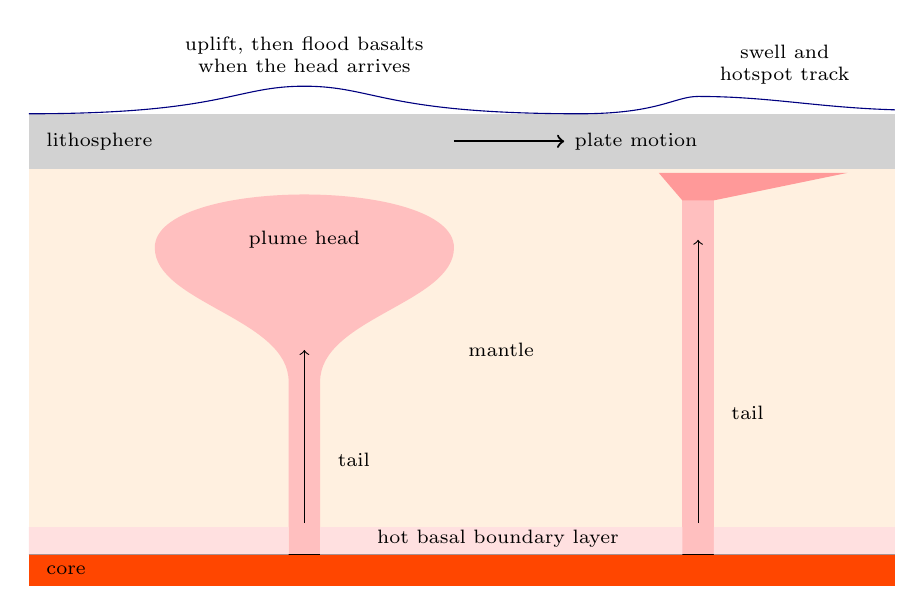
\begin{tikzpicture}[font=\scriptsize, x=1cm, y=1cm]
\fill[orange!12] (0,0) rectangle (11,-5.6);
\fill[gray!35] (0,0) -- (11,0) -- (11,-0.7) -- (0,-0.7) -- cycle;
\fill[red!25] (3.3,-5.6) -- (3.3,-3.4) .. controls (3.3,-2.6) and (1.6,-2.4) .. (1.6,-1.7)
  .. controls (1.6,-0.8) and (5.4,-0.8) .. (5.4,-1.7) .. controls (5.4,-2.4) and (3.7,-2.6) .. (3.7,-3.4) -- (3.7,-5.6) -- cycle;
\fill[red!25] (8.3,-5.6) -- (8.3,-0.75) -- (8.7,-0.75) -- (8.7,-5.6) -- cycle;
\fill[red!40] (8.0,-0.75) -- (8.3,-1.1) -- (8.7,-1.1) -- (10.4,-0.75) -- cycle;
\draw[thick] (0,-5.6) -- (11,-5.6);
\fill[red!45!orange] (0,-5.6) rectangle (11,-6.0);
\fill[red!12] (0,-5.6) rectangle (3.3,-5.25) (3.7,-5.6) rectangle (8.3,-5.25) (8.7,-5.6) rectangle (11,-5.25);
\node[anchor=west] at (0.1,-5.8) {core};
\node at (3.5,-1.6) {plume head};
\node[anchor=west] at (3.8,-4.4) {tail};
\node[anchor=west] at (8.8,-3.8) {tail};
\node[anchor=west] at (0.1,-0.35) {lithosphere};
\node at (6.0,-3.0) {mantle};
\draw[->] (3.5,-5.2) -- (3.5,-3.0);
\draw[->] (8.5,-5.2) -- (8.5,-1.6);
\draw[->, thick] (5.4,-0.35) -- (6.8,-0.35) node[right] {plate motion};
\draw[blue!50!black] (0,0) .. controls (2.5,0) and (2.6,0.35) .. (3.5,0.35) .. controls (4.4,0.35) and (4.5,0) .. (7,0) .. controls (8,0) and (8.2,0.22) .. (8.5,0.22) .. controls (9.4,0.22) and (10,0.08) .. (11,0.05);
\node[above, align=center] at (3.5,0.4) {uplift, then flood basalts\\when the head arrives};
\node[above, align=center] at (9.6,0.25) {swell and\\hotspot track};
\node[anchor=west] at (4.3,-5.4) {hot basal boundary layer};
\end{tikzpicture}

\par\smallskip{\small A young plume (left) rises as a large head fed by a thin
tail; when the head spreads beneath the lithosphere, the surface rises and flood
basalts may erupt. An older plume (right) is a tail beneath a moving plate,
feeding a swell and a hotspot track. Not to
scale.}\label{fig:b3:mantle-convection:plume}
\end{omfigure}

A plume head is a sphere of buoyant mantle rising through the viscous mantle:
physics' Stokes law, $v = 2\Delta\rho\,ga^2/(9\eta)$, gives its speed in order of
magnitude, a fraction of a metre a year for a head a few hundred kilometres
across (exercise 8), so that it crosses the mantle in millions of years.

\section{Glacial isostatic adjustment and the viscosity of the mantle}\label{sec:b3:mantle-convection:gia}

\begin{definition}[Glacial isostatic adjustment, mantle viscosity]\label{def:b3:mantle-convection:gia}
\emph{Glacial isostatic adjustment}\index{glacial isostatic adjustment} (GIA)
is the slow deformation of the solid Earth, and the change of its gravity
field and of sea level, as it returns towards isostatic equilibrium after an
ice sheet grows or melts. The \emph{mantle viscosity}\index{mantle viscosity}
is the effective viscosity $\eta$ that relates the slow, steady creep of the
mantle to the stresses that drive it, over times of thousands of years and more.
\end{definition}

When an ice sheet melts, the depression it leaves is out of isostatic
equilibrium: beneath it, the mantle's pressure is lower than around it, and
mantle flows in to lift the floor back. Today the coast of the Gulf of Bothnia
rises at up to \qty{10.3}{mm/yr}, near Umeå; Hudson Bay at about
\qty{10}{mm/yr}, where the ice was thickest, while the land south of the Great
Lakes sinks by 1 to \qty{2}{mm/yr}, as the bulge that the ice had pushed up
around it subsides. On the coasts, old shorelines now stand above the sea, the
raised beaches of the field box below.
% ledger: vestol19:umea, sella07:gia

\begin{theorem}[Relaxation of a viscous half-space]\label{thm:b3:mantle-convection:relaxation}
A depression $w(x, t) = w_m(t)\cos(2\pi x/\lambda)$ of the surface of a
half-space of uniform viscosity $\eta$ and density $\rho$, left without load,
decays as $w_m(t) = w_m(0)e^{-t/\tau}$ with
\[
  \tau = \frac{4\pi\eta}{\rho g\lambda} .
\]
\end{theorem}

\begin{proof}
Take $z$ downwards, $k = 2\pi/\lambda$, and look for a Stokes flow that decays
with depth, with vertical velocity (downwards) $v = (C + Dkz)e^{-kz}\cos kx$.
Incompressibility gives the horizontal velocity $u = -(D - C - Dkz)e^{-kz}\sin
kx$. These functions satisfy $\nabla^4 = 0$, as every Stokes flow in two
dimensions does. The free surface carries no shear stress: $\partial u/\partial
z + \partial v/\partial x = 2k(D - C)\sin kx = 0$ at $z = 0$, so $D = C$, and
\[
  v = C(1 + kz)e^{-kz}\cos kx,\quad u = Ckze^{-kz}\sin kx,\quad
  p = 2\eta Cke^{-kz}\cos kx,
\]
the pressure following from $\partial p/\partial x = \eta\nabla^2u = -2\eta
Ck^2e^{-kz}\sin kx$ (and $\partial p/\partial z = \eta\nabla^2v$ checks). At the
surface $\partial v/\partial z = 0$, so the normal stress there is $-p$. Beneath
a depression $w$, the weight of the missing rock lowers the pressure by $\rho
gw$: $p(0) = -\rho gw$, so $2\eta Ck = -\rho gw_m$. The surface moves with the
fluid: $\mathrm dw_m/\mathrm dt = v(0) = C = -\rho gw_m/(2\eta k)$, whose
solution decays with $\tau = 2\eta k/(\rho g) = 4\pi\eta/(\rho g\lambda)$.
\end{proof}

\begin{definition}[Isostatic relaxation time]\label{def:b3:mantle-convection:relaxation-time}
The \emph{isostatic relaxation time}\index{isostatic relaxation time} $\tau$ of
a load of horizontal scale $\lambda$ is the time in which its departure from
isostatic equilibrium decays by the factor $e$.
\end{definition}

A uniform half-space relaxes broad depressions faster than narrow ones, and the
flow beneath a load of wavelength $\lambda$ decays with depth as $e^{-kz}$, over
a depth $\lambda/2\pi$: a large ice sheet stirs the mantle deeply, a small lake
only its top. For a depression \qty{3000}{km} across and $\eta =
\qty{e21}{Pa.s}$, with $\rho = \qty{3300}{kg.m^{-3}}$, $\tau = \qty{4.1}{kyr}$
(figure below): after ten thousand years, $e^{-2.4} = \qty{9}{\percent}$ of
the depression remains, and since $\dot w = -w/\tau$, an uplift of
\qty{10}{mm/yr} means that some \qty{40}{m} of rise are still to come.

\begin{omfigure}
\begin{tikzpicture}
\begin{groupplot}[group style={group size=1 by 2, vertical sep=2.5cm},
  omrecord, width=0.86\linewidth, height=0.38\linewidth]
\nextgroupplot[xmin=0, xmax=20, ymin=0, ymax=1.05, xlabel={time since the ice melted (kyr)},
  ylabel={$w_m(t)/w_m(0)$}, title={(a) decay of a depression \qty{3000}{km} across},
  title style={font=\small}, legend style={font=\scriptsize, at={(0.98,0.97)}, anchor=north east}]
% computed in figdata/bachelor-3/gia_relaxation.py; ledger: mitrovica96:haskell, milne04:bifrost
\addplot[red!70!black, thick, densely dashed] table[x=t, y=f20] {figdata/out/bachelor-3-gia_relaxation-decay.dat};
\addlegendentry{$\eta = \qty{e20}{Pa.s}$}
\addplot[omDef, thick] table[x=t, y=f21] {figdata/out/bachelor-3-gia_relaxation-decay.dat};
\addlegendentry{$\eta = \qty{e21}{Pa.s}$}
\addplot[black, thick, densely dotted] table[x=t, y=f22] {figdata/out/bachelor-3-gia_relaxation-decay.dat};
\addlegendentry{$\eta = \qty{e22}{Pa.s}$}
\nextgroupplot[xmode=log, ymode=log, xmin=100, xmax=1e4, ymin=0.01, ymax=1000,
  xlabel={wavelength $\lambda$ (km)}, ylabel={$\tau$ (kyr)},
  title={(b) relaxation time against wavelength}, title style={font=\small}]
\addplot[red!70!black, thick, densely dashed] table[x=lam, y=t20] {figdata/out/bachelor-3-gia_relaxation-tau.dat};
\addplot[omDef, thick] table[x=lam, y=t21] {figdata/out/bachelor-3-gia_relaxation-tau.dat};
\addplot[black, thick, densely dotted] table[x=lam, y=t22] {figdata/out/bachelor-3-gia_relaxation-tau.dat};
\end{groupplot}
\end{tikzpicture}

\par\smallskip{\small Relaxation of a uniform viscous half-space ($\rho =
\qty{3300}{kg.m^{-3}}$, $g = \qty{9.8}{m.s^{-2}}$) for three viscosities. (a) The
fraction of the depression left with time. (b) The relaxation time
$4\pi\eta/(\rho g\lambda)$, longer for narrow loads.}\label{fig:b3:mantle-convection:gia}
\end{omfigure}

The real mantle is not uniform, and its rebound is read with models that layer
it and add an elastic lithosphere, which holds up narrow loads by flexure. The
first estimate, from the rebound of Fennoscandia, gave \qty{e21}{Pa.s}, and the
decay of uplift at the Angerman River in Sweden and at Richmond Gulf on Hudson
Bay gives an average of 0.65 to \qty{1.1e21}{Pa.s} from the base of the
lithosphere down to about \qty{1400}{km}, with the upper mantle about ten times
less viscous than the lower. Inversions of the GNSS uplift rates of
Fennoscandia give upper-mantle viscosities of \num{5e20} to \qty{e21}{Pa.s}
in one study and \num{3.4e20} to \qty{5.0e20}{Pa.s} in another, lower-mantle
viscosities of \num{5e21} to \qty{5e22}{Pa.s}, and a lithosphere 93 to
\qty{110}{km} thick. The estimates differ by factors of two or three, but they
agree on the order of magnitude and on the increase with depth.
% ledger: mitrovica96:haskell, milne04:bifrost, zhao12:fenno

\begin{definition}[Maxwell time]\label{def:b3:mantle-convection:maxwell}
The \emph{Maxwell time}\index{Maxwell time} of a material of viscosity $\eta$
and shear modulus $\mu$ is $\tau_M = \eta/\mu$: loads applied for much less than
$\tau_M$ meet an elastic solid, loads applied for much longer a viscous fluid.
\end{definition}

With $\mu = \rho v_S^2 = \qty{7.7e10}{Pa}$ at \qty{300}{km} in PREM and $\eta =
\qty{e21}{Pa.s}$, $\tau_M = \qty{1.3e10}{s}$, about four hundred years. A
seismic wave, which lasts seconds, crosses an elastic mantle; an ice age, and
convection, deform a fluid one. The same rock is both, depending on how long it
is pushed.
% ledger: data:prem

\begin{inthefield}[Raised beaches]
\begin{minipage}[t]{0.55\linewidth}\vspace{0pt}
On the coasts of formerly glaciated lands, a geomorphologist finds the sea's
old work stranded inland: ridges of rounded shingle, notches and flat
platforms cut by waves, now standing above the reach of today's highest
tides, sometimes in a staircase of several levels. Each level was a shoreline
when the sea stood there; the land has risen since. Shells and driftwood in
the old beaches are dated by radiocarbon, and the heights of the dated levels,
levelled to a benchmark, give the uplift against time. Traced along a coast,
an old shoreline is found to slope, highest where the ice was thickest: the
tilt maps the shape of the rebound.
\end{minipage}\hfill
\begin{minipage}[t]{0.42\linewidth}\vspace{0pt}
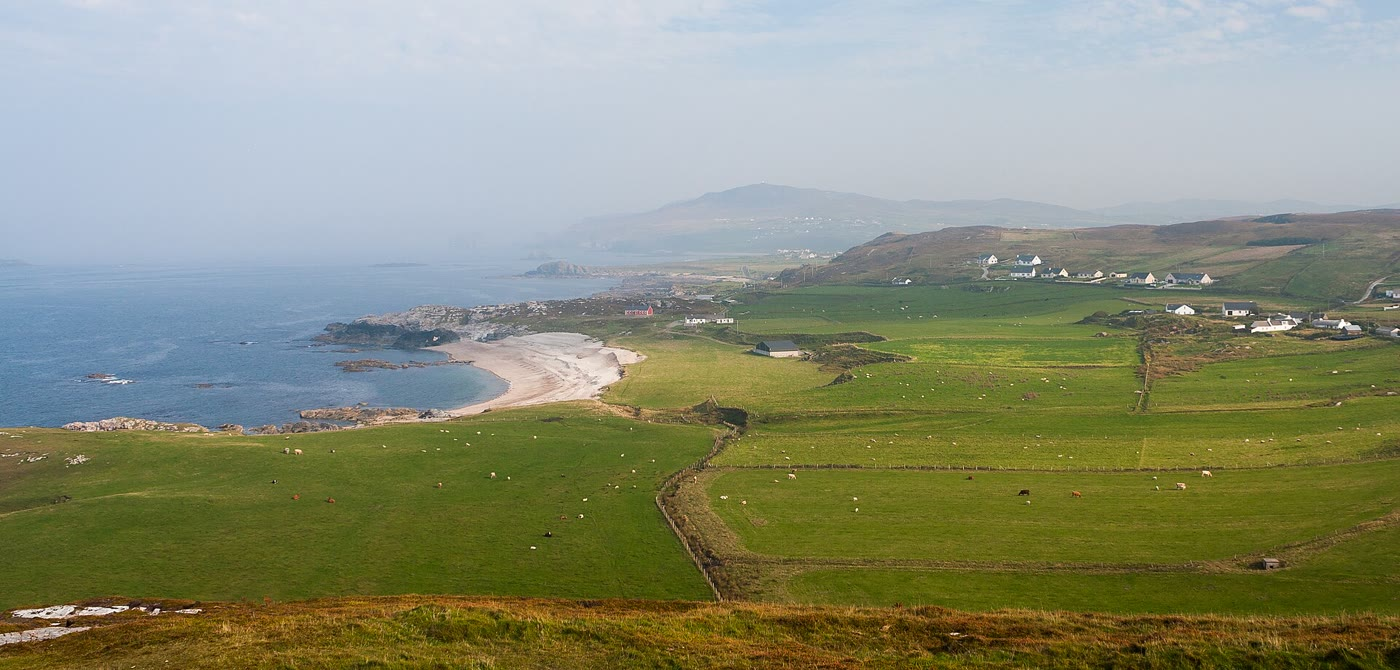
\includegraphics[width=\linewidth]{images/book5/b3-raised-beach-malin.jpg}

{\scriptsize The raised beaches of Ballyhillin, Malin Head, in the north of
Ireland: shingle ridges of old shorelines lifted above the sea as the land rose
after its ice sheet melted. Photo A.~F.~Borchert, CC BY-SA 4.0.}
\end{minipage}
\end{inthefield}
% ledger: photo:b3-raised-beach

\section{Whole-mantle convection and its deep structure}

Does the mantle convect as one layer, or as two, above and below the
\qty{670}{km} discontinuity? Tomography (\cref{ch:b3:seismology-imaging})
answers in part: some slabs flatten above the discontinuity, others plunge
through it into the lower mantle, so mass crosses it and the two layers are not
sealed from each other. The increase of viscosity with depth makes the lower
mantle flow more sluggishly, and slabs slow and thicken as they enter it.

At the base of the mantle, tomography shows two broad regions of low S-wave
speed, beneath Africa and beneath the Pacific, the large low-shear-velocity
provinces (LLSVPs). They are probably chemically distinct from the mantle above
them and denser, piles rather than hot plumes. The large igneous provinces and
kimberlites of the last few hundred million years erupted mostly above their
margins, as if plumes rose from the edges of the piles, where the hot boundary
layer at the base of the mantle is swept against them.
% ledger: st12:llsvp

\section{Exercises}

\begin{exercise}[$\star$]\label{exo:b3:mantle-convection:1}
Compute the \omterm{def:b3:mantle-convection:rayleigh}{Rayleigh number} of an upper-mantle layer \qty{670}{km} thick with
$\rho = \qty{3500}{kg.m^{-3}}$, $g = \qty{9.9}{m.s^{-2}}$, $\alpha =
\qty{3e-5}{K^{-1}}$, $\Delta T = \qty{1000}{K}$, $\kappa =
\qty{e-6}{m^2.s^{-1}}$ and $\eta = \qty{5e20}{Pa.s}$. How many times critical is
it, for free-slip boundaries?
\end{exercise}

\begin{exercise}[$\star$]\label{exo:b3:mantle-convection:2}
Compute the \omterm{def:b3:mantle-convection:maxwell}{Maxwell time} of a mantle of viscosity \qty{e21}{Pa.s} and shear
modulus \qty{7.7e10}{Pa}, in years. Does the mantle respond elastically or
viscously to the twice-daily Earth tide, to the melting of an ice sheet, and to
the sinking of a slab?
\end{exercise}

\begin{exercise}[$\star$]\label{exo:b3:mantle-convection:3}
With $\eta = \qty{e21}{Pa.s}$, $\rho = \qty{3300}{kg.m^{-3}}$ and $g =
\qty{9.8}{m.s^{-2}}$, compute the relaxation time of a uniform half-space for
loads of wavelength 1000 and \qty{3000}{km}. Which recovers faster?
\end{exercise}

\begin{exercise}[$\star$]\label{exo:b3:mantle-convection:4}
With $g = \qty{9.8}{m.s^{-2}}$, $\rho_m = \qty{3300}{kg.m^{-3}}$, $\rho_w =
\qty{1030}{kg.m^{-3}}$, $\alpha = \qty{3.1e-5}{K^{-1}}$, $T_m - T_0 =
\qty{1450}{K}$, $\kappa = \qty{0.8e-6}{m^2.s^{-1}}$ and \qty{1}{Myr} $=
\qty{3.156e13}{s}$, compute the \omterm{prop:b3:mantle-convection:ridge-push}{ridge-push force} at \qty{50}{Myr}. How many times
smaller is it than a slab pull of \qty{4.6e13}{N.m^{-1}}?
\end{exercise}

\begin{exercise}[$\star\star$]\label{exo:b3:mantle-convection:5}
A blob of mantle \qty{10}{km} across, \qty{300}{K} hotter than its
surroundings, rises at the speed $\rho g\alpha\Delta Td^2/\eta$ (take $\rho =
\qty{3300}{kg.m^{-3}}$, $g = \qty{9.8}{m.s^{-2}}$, $\alpha = \qty{3e-5}{K^{-1}}$,
$\eta = \qty{e21}{Pa.s}$, $\kappa = \qty{e-6}{m^2.s^{-1}}$). (a) Compute its
rise time across its own size and its diffusion time $d^2/\kappa$, and show
that their ratio is its \omterm{def:b3:mantle-convection:rayleigh}{Rayleigh number}. (b) Does it rise or cool first? (c)
How large must it be for its \omterm{def:b3:mantle-convection:rayleigh}{Rayleigh number} to reach 657.5?
\end{exercise}

\begin{exercise}[$\star\star$]\label{exo:b3:mantle-convection:6}
For a layer \qty{2891}{km} deep at $\mathrm{Ra} = \num{e7}$, with $\kappa =
\qty{e-6}{m^2.s^{-1}}$, $k = \qty{3.1}{W.m^{-1}.K^{-1}}$, $\Delta T =
\qty{1450}{K}$ and $\mathrm{Ra}_c = 657.5$, compute the boundary-layer
thickness, the \omterm{def:b3:mantle-convection:nusselt}{Nusselt number}, the velocity scale in \unit{cm/yr} and the heat
flow.
\end{exercise}

\begin{exercise}[$\star\star$]\label{exo:b3:mantle-convection:7}
An invented hotspot swell has a cross-sectional area of \qty{8e8}{m^2} across
the track, and the plate above moves at \qty{9}{cm/yr}. With $\rho_m - \rho_w =
\qty{2270}{kg.m^{-3}}$, compute its buoyancy flux, and its heat flux with $c_p =
\qty{1170}{J.kg^{-1}.K^{-1}}$ and $\alpha = \qty{3.1e-5}{K^{-1}}$. What fraction
of the Earth's \qty{46.7}{TW} is it?
\end{exercise}

\begin{exercise}[$\star\star$]\label{exo:b3:mantle-convection:8}
A plume head of radius \qty{400}{km}, lighter than the mantle by
\qty{30}{kg.m^{-3}}, rises through a mantle of viscosity \qty{e21}{Pa.s}. With
Stokes' law, compute its speed in \unit{m/yr} and the time it takes to rise
\qty{2000}{km}.
\end{exercise}

\begin{exercise}[$\star\star$]\label{exo:b3:mantle-convection:9}
A region was depressed by \qty{300}{m} when its ice melted, \qty{10}{kyr} ago,
and relaxes with $\tau = \qty{4.4}{kyr}$. Compute the depression left today and
the present uplift rate. Compare with the \qty{10.3}{mm/yr} measured near
Umeå.
\end{exercise}

\begin{exercise}[$\star\star\star$]\label{exo:b3:mantle-convection:10}
(a) From the expression of $F_{rp}$ in the proof of
\cref{prop:b3:mantle-convection:ridge-push}, show that the first term,
$\tfrac12(\rho_m - \rho_w)gw^2$, is the second term of the bracket. (b) Show that
$\int_0^\infty x\operatorname{erfc}x\,\mathrm dx = 1/4$, by integrating by parts.
(c) With the values of exercise 4, compute the two terms at \qty{100}{Myr}.
\end{exercise}

\begin{exercise}[$\star\star\star$]\label{exo:b3:mantle-convection:11}
Show that $f(k) = (\pi^2 + k^2)^3/k^2$ is smallest at $k = \pi/\sqrt2$, where
it equals $27\pi^4/4$. Deduce the width of a pair of convection cells at onset,
in units of $d$, and the width of one cell.
\end{exercise}

\begin{exercise}[$\star\star\star$]\label{exo:b3:mantle-convection:12}
A plate \qty{6000}{km} long moves at \qty{6}{cm/yr} over a mantle layer
\qty{150}{km} thick, of viscosity \qty{e20}{Pa.s}, whose base is at rest. (a)
Compute the \omterm{def:b3:mantle-convection:basal-drag}{basal drag} in \unit{MPa} and the drag force per unit length of plate.
(b) Compare with a ridge push of \qty{3.8e12}{N.m^{-1}} and a slab pull of
\qty{4.6e13}{N.m^{-1}}. (c) If one tenth of the slab pull reaches the plate,
at what speed does the drag balance the driving forces?
\end{exercise}

\section{Problem: Rebound of Lake Ardo}

\begin{problem}[{Weekend problem --- the rebound of an invented lake basin,
the viscosity of the mantle beneath it, and the convection that viscosity
allows}]
\label{pb:b3:mantle-convection:1}
% values: calc/ch06.py; gia_relaxation.py, convection_scaling.py
Lake Ardo, an invented lake, filled a basin \qty{250}{km} across, dammed by an
ice sheet, and stood \qty{300}{m} deep for about fifty thousand years. Fourteen
thousand years ago the ice dam failed and the lake drained in a few weeks. Its
highest shoreline, level when it formed, is now tilted; dated shorelines of
the small lakes left in the basin give the uplift of the centre since the
drainage, relative to the rim, which barely moved:

\smallskip
\begin{center}\small
\begin{tabular}{lcccccc}
\hline
time since the drainage (kyr) & 1 & 2 & 4 & 6 & 9 & 14\\
uplift of the centre (m) & 11.5 & 21.6 & 38.0 & 50.5 & 64.0 & 77.2\\
\hline
\end{tabular}
\end{center}
\smallskip

Take $\rho_w = \qty{1000}{kg.m^{-3}}$, $\rho_m = \qty{3300}{kg.m^{-3}}$, $g =
\qty{9.8}{m.s^{-2}}$, \qty{1}{yr} $= \qty{3.156e7}{s}$, and treat the mantle as
a uniform viscous half-space.

\medskip\noindent\textbf{Part I --- The load.}
\begin{enumerate}
  \item Compute the pressure of the lake on its floor.
  \item Compute the depression of the floor at isostatic equilibrium, and say
        why the density of the mantle, not of the crust, appears in it.
  \item Treating the lake as a disc, compute the mass of its water.
  \item Explain why the highest shoreline is now tilted, and compute its mean
        slope from the rim to the centre, in metres per kilometre.
  \item The depression is treated as one harmonic whose depressed half, from
        $-\lambda/4$ to $\lambda/4$, spans the lake. Give $\lambda$ and $k =
        2\pi/\lambda$.
  \item Over what depth does the flow beneath such a load decay by the factor
        $e$?
\end{enumerate}

\medskip\noindent\textbf{Part II --- The relaxation time.}
\begin{enumerate}[resume]
  \item Assuming the lake had reached equilibrium, compute the depression left
        at each date of the table.
  \item Show that, if the depression decays exponentially, its logarithm falls
        linearly with time.
  \item Compute $\tau$ from the dates 1 and \qty{14}{kyr}.
  \item Predict the uplift at \qty{6}{kyr} with that $\tau$ and compare with the
        table.
  \item Compute the depression left today and the present uplift rate of the
        centre, in \unit{mm/yr}.
  \item How much uplift is still to come?
  \item In how many more years will the uplift rate fall below
        \qty{0.5}{mm/yr}?
\end{enumerate}

\medskip\noindent\textbf{Part III --- The viscosity.}
\begin{enumerate}[resume]
  \item Compute the viscosity of the half-space from $\tau$.
  \item Compare it with the upper-mantle viscosities of \num{3.4e20} to
        \qty{1e21}{Pa.s} found beneath Fennoscandia. Which part of the mantle
        does the rebound of Lake Ardo sample?
  \item With that viscosity, compute the relaxation time of a load
        \qty{3000}{km} in wavelength. Why would a real ice sheet of that size
        relax more slowly than this?
  \item What does an elastic lithosphere, ignored here, do to the rebound of a
        load only \qty{250}{km} across?
  \item Compute the \omterm{def:b3:mantle-convection:maxwell}{Maxwell time} of the mantle with $\mu = \qty{7.7e10}{Pa}$,
        and say whether a viscous model was justified.
  \item Check the assumption of question 7: what fraction of the equilibrium
        depression was reached while the lake stood?
  \item By how much would $\log_{10}\eta$ change if $\lambda$ were taken as
        \qty{250}{km}?
\end{enumerate}

\medskip\noindent\textbf{Part IV --- Convection.} Take an upper-mantle layer
\qty{670}{km} deep with $\rho = \qty{3700}{kg.m^{-3}}$, $g =
\qty{9.9}{m.s^{-2}}$, $\alpha = \qty{3.1e-5}{K^{-1}}$, $\Delta T =
\qty{1450}{K}$, $\kappa = \qty{e-6}{m^2.s^{-1}}$, $k = \qty{3.1}{W.m^{-1}.K^{-1}}$
and the viscosity of Part III.
\begin{enumerate}[resume]
  \item Compute the \omterm{def:b3:mantle-convection:rayleigh}{Rayleigh number} of the layer.
  \item How many times critical is it ($\mathrm{Ra}_c = 657.5$)?
  \item Compute the boundary-layer thickness and the \omterm{def:b3:mantle-convection:nusselt}{Nusselt number}.
  \item Compute the velocity scale in \unit{cm/yr}, and compare with plate
        speeds of 1 to \qty{7.5}{cm/yr}.
  \item Compute the heat flow, and give two reasons why it falls short of the
        Earth's mean, \qty{92}{mW.m^{-2}}.
  \item Give the upper-mantle viscosity beneath Lake Ardo as $\log_{10}$ of
        $\eta$ in \unit{Pa.s}.
\end{enumerate}
\end{problem}
